\subsection{The scheme equation}
We now move on to the scalar linear advection equation with positive coefficients $s_1,s_2>0$.
Moreover, the space coordinates $x_1,x_2$ in the ($\vect{e}_1,\vect{e}_2$) plane are written $x$ and $y$.
Then, the physical domain under consideration, that is $x,y \in [0,l]\times[0,h]$, is discretized with $N_p$ material points arbitrarily distributed in a Cartesian grid made of $E$ four-node bilinear elements with constant size $\Delta x \times \Delta y$.
\begin{figure}[h!]
  \centering
  \begin{tikzpicture}
  \draw[thick,->] (-1.5,0.)--(1.5,0.) node [right] {$\xi$};
  \draw[thick,->] (0.,-1.5)--(0.,1.5) node [above] {$\eta$};
  \draw (-1.,-1.0) rectangle (1.,1.);
  \node[above right] at (0.,1.) {$1$};\node[above right] at (0.,-1.) {-$1$};
  \node[above right] at (-1,0.) {-$1$};\node[above right] at (1.,.) {$1$};
  \draw[thick,->] (-.25+5.,0.)--(1.5+5.,0.) node [right] {$X$};
  \draw[thick,->] (0.+5.,-.25)--(0.+5.,1.5) node [above] {$Y$};
  % origin at (+5.,0.)
  \draw (6.,1.) node [below] {$X_1$}-- (8.,1.5) node [below] {$X_2$}-- (9.,4.) node [above] {$X_3$}-- (6.5,3.5) node [above] {$X_4$}-- (6.,1.);
  \fill[black] (8.,3.25) circle (0.05) node [above] {$\vect{X}$};
  \fill[black] (.5,.5) circle (0.05) node [above] {$\vect{\xi}$};
  \draw[->] (8.,3.25) .. controls (6.,3.25) and (1.5,1.5) .. (.5,.5);
\end{tikzpicture}
  
  \caption{Parent and current configuration of a rectangular four-node bilinear element}
  \label{fig:2Dparent}
\end{figure}
With positions of nodes of cell $C$ denoted by $\vect{x}_i^C=\matrice{x^C_i \\ y_i^C}$, as depicted in figure \ref{fig:2Dparent}, the location $\vect{x}$ of an arbitrary point in cell $C$ maps to the parent coordinates $(\xi,\eta)$ in the domain $\[-1,1\]\times\[-1,1\]$ according to:
\begin{equation}
  \label{eq:parentCoordinates}
  \begin{aligned}
      &\xi = 2\frac{x-x^C_1}{\Delta x} -1 \quad ; \quad d\xi = 2\frac{dx}{\Delta x} \\
      &\eta = 2\frac{y-y^C_1}{\Delta y} -1 \quad ; \quad d\eta = 2\frac{dy}{\Delta y} 
  \end{aligned}
\end{equation}
Horizontal and vertical edges lengths are distinguished here in spite of the Cartesian nature of the grid in order to easily extend the following study to rectilinear grids. Again, there is no empty cell inside the physical domain so that no hole is generated, and periodic boundary conditions are considered to simplify the analysis.
Though, one can imagine to combine the DGMPM discretization with a multi-stage time integration as proposed for one-dimensional problems, the equations one has to deal with become complicated.
Hence, the analysis of the DGMPM scheme for two-dimensional problems carried out here only considers the Euler time discretization.

The updated solution at material point $I$ is obtained by interpolation of updated nodal quantities:
\begin{equation}
  \label{eq:2D_updatedMP}
  \bar{Q}^{k+1}_I = \sum_{i=1}^{4E}S_{iI} \bar{q}_i^{k+1}
\end{equation}
where the $\bar{q}_i^{k+1}$ result from the discrete system:
\begin{equation}
  \bar{q}_i^{k+1} = \bar{q}_i^k + \frac{\Delta t}{M^L_i} \(K_{ij}^x s_1\bar{q}_j^k + K_{ij}^y s_2\bar{q}_j^k - \hat{F}^k_i\) \label{eq:discrete2D}
\end{equation}

The lumped mass matrix in the above equation has the same expression as in the one-dimensional case that depends on the shape functions of the four-node bilinear element: $M_i^L=\sum_K m_K S_{iK}$.
Making use of parent coordinates \eqref{eq:parentCoordinates}, the pseudo-stiffness matrices read:
\begin{equation}
  \begin{aligned}
    & K_{ij}^x = \sum_J \drond{S_{iJ}}{x}m_J S_{jJ}=\frac{2}{\Delta x}\sum_J\drond{S_{iJ}}{\xi}m_J S_{jJ} \\
    &K_{ij}^y = \sum_J\drond{S_{iJ}}{y}m_J S_{jJ}=\frac{2}{\Delta y}\sum_J\drond{S_{iJ}}{\eta}m_J S_{jJ} \\
  \end{aligned}
\end{equation}
As for one-dimensional cases, the homogeneous medium yields the same mass for every particles so that, by writing $\drond{(\bullet)}{\xi}=\partial_\xi(\bullet)$, one gets:
\begin{equation}
  \label{eq:2Dpseudo_stiffness}
  \begin{aligned}
    & \frac{K_{ij}^x}{M_i^L}  =  \frac{2}{\Delta x} \frac{\sum_J\partial_\xi S_{iJ}  S_{jJ}}{\sum_K  S_{iK}} \\
    & \frac{K_{ij}^y}{M_i^L} = \frac{2}{\Delta y} \frac{\sum_J\partial_\eta S_{iJ} S_{jJ}}{\sum_K S_{iK}}
  \end{aligned}
\end{equation}
The nodal solutions in cell $C$ at time $k$ being given by the projection $\bar{q}^{C,k}_i=\frac{\sum_L S_{iL}\bar{Q}^k_L}{\sum_K S_{iK}}$, volume fluxes of the discrete form can be rewritten as:
\begin{equation}
  \label{eq:2Dvolume_fluxes}
  \begin{aligned}
    & s_1\frac{K_{ij}^x}{M_i^L}\bar{q}^k_j  = \sum_L\bar{Q}^k_L\frac{2}{\Delta x} \frac{s_1\sum_J\partial_\xi S_{iJ}  \sum_j S_{jJ} S_{jL}}{\sum_K S_{iK}\sum_K S_{jK}}\\
    & s_2\frac{K_{ij}^y}{M_i^L}\bar{q}^k_j = \sum_L \bar{Q}^k_L\frac{2}{\Delta y}  \frac{s_2 \sum_J\partial_\eta S_{iJ}  \sum_j S_{jJ} S_{jL}}{\sum_K  S_{iK}\sum_K S_{jK}}
  \end{aligned}
\end{equation}
Then, the nodal interface flux $\hat{F}^k_i$ results from the integration of Godunov's fluxes along edges the node belongs to, according to the weak form \eqref{eq:DGMPM_semi_discrete}.
Referring to a quantity defined at an interface by means of parenthesis superscripts, the Godunov's flux at interface $(i)$ is:
\begin{equation}
  \label{eq:2d_Godunov_fluxes}
  F_n^{(i)}= s_n q^{-,(i)} = \underbrace{s_nq^{+,(i)}}_{F_n(q^{+,(i)})} - \underbrace{s_n (q^{+,(i)}-q^{-,(i)} )}_{\Ac^{+}_{U/D}} 
\end{equation}
where $s_n$ is the speed in the normal direction to the interface (\textit{i.e. $s_2$ for horizontal edges and $s_1$ for vertical edges}). Equation \eqref{eq:2d_Godunov_fluxes} further involves state vectors $q^{-,(i)}$ and $q^{+,(i)}$ obtained by averaging nodal values connected to interface $(i)$ on Upwind and Downwind sides respectively, and the right-going fluctuation $\Ac_{U/D}^+$.
The CTU is adopted by adding transverse corrections to fluxes \eqref{eq:2d_Godunov_fluxes}, based on those fluctuations according to equation \eqref{eq:corrected_flux}:
\begin{equation}
  \label{eq:2D_transverse_corrections}
  \Bc^+\Ac^+_{U/D}=s_t s_n (q^{+,(i)} -q^{-,(i)})
\end{equation}
with $s_t$ the speed in the tangent direction to the interface. The final expression of intercell fluxes is hence:
\begin{equation}
  \label{eq:CTU-fluxes}
  F_n^{(i)}= s_n q^{-,(i)} - s_t s_n \frac{\Delta t}{2\Delta x}(q^{+,(i)} -q^{-,(i)})
\end{equation}
\begin{figure}[h!]
  \centering
  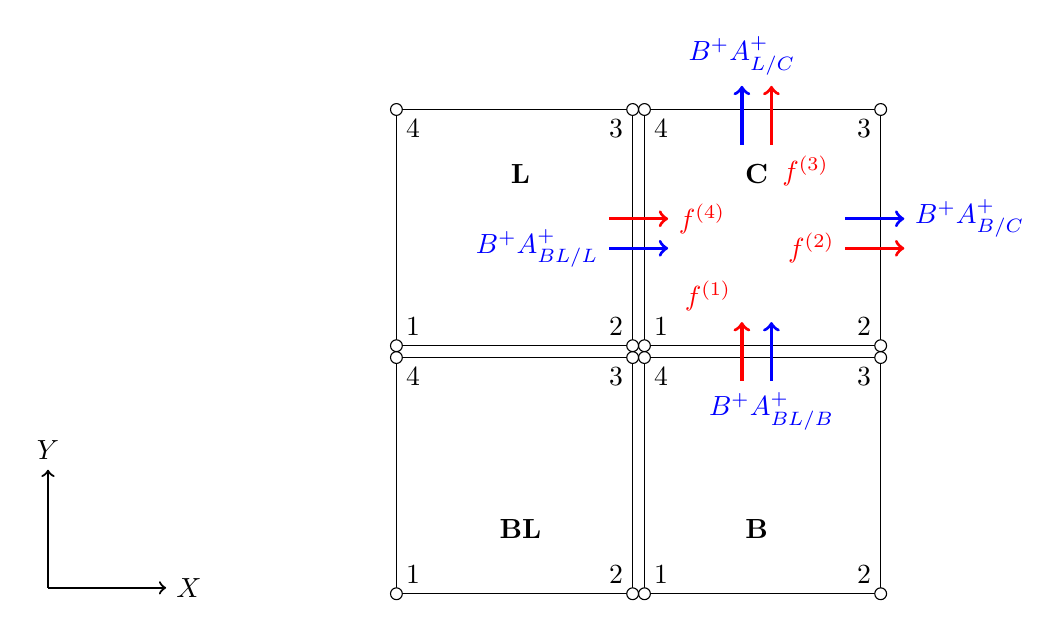
\begin{tikzpicture}[scale=1.5]
  \draw[thick,->] (-3,0.)-- (-2,0.) node[right] {$X$};
  \draw[thick,->] (-3,0.)-- (-3,1.) node[above] {$Y$};

  %% Cells
  \draw (0-0.05,0-0.05) rectangle (2.-0.05,2-0.05);
  \draw (0-0.05,2+0.05) rectangle (2.-0.05,4+0.05);
  \draw (2+0.05,0-0.05) rectangle (4.+0.05,2-0.05);
  \draw (2+0.05,2+0.05) rectangle (4.+0.05,4+0.05);
  %%%%%%%%%%%%%%%%%%%%%
  
  %% Nodes
  \fill[white] (0-0.05,0-0.05) circle (0.05);\fill[white] (2-0.05,2-0.05) circle (0.05);
  \fill[white] (0-0.05,2+0.05) circle (0.05);\fill[white] (2.-0.05,4+0.05) circle (0.05);
  \fill[white] (2+0.05,0-0.05) circle (0.05);\fill[white] (4.+0.05,2-0.05) circle (0.05);
  \fill[white] (2+0.05,2+0.05) circle (0.05);\fill[white] (4.+0.05,4+0.05) circle (0.05);
  \fill[white] (2-0.05,0-0.05) circle (0.05);\fill[white] (4.+0.05,0-0.05) circle (0.05);
  \fill[white] (0-0.05,2-0.05) circle (0.05);\fill[white] (2.+0.05,2-0.05) circle (0.05);
  \fill[white] (2-0.05,2+0.05) circle (0.05);\fill[white] (4.+0.05,2.+0.05) circle (0.05);
  \fill[white] (-0.05,4+0.05) circle (0.05);\fill[white] (2.+0.05,4+0.05) circle (0.05);

  \draw (0-0.05,0-0.05) circle (0.05) node[above right] {$1$};\draw (2-0.05,2-0.05) circle (0.05) node[below left] {$3$};
  \draw (0-0.05,2+0.05) circle (0.05) node[above right] {$1$};\draw (2.-0.05,4+0.05) circle (0.05) node[below left] {$3$};
  \draw (2+0.05,0-0.05) circle (0.05) node[above right] {$1$};\draw (4.+0.05,2-0.05) circle (0.05) node[below left] {$3$};
  \draw (2+0.05,2+0.05) circle (0.05) node[above right] {$1$};\draw (4.+0.05,4+0.05) circle (0.05) node[below left] {$3$};
  \draw (2-0.05,0-0.05) circle (0.05) node[above left] {$2$};\draw (4.+0.05,0-0.05) circle (0.05) node[above left] {$2$};
  \draw (0-0.05,2-0.05) circle (0.05) node[below right] {$4$};\draw (2.+0.05,2-0.05) circle (0.05) node[below right] {$4$};
  \draw (2-0.05,2+0.05) circle (0.05) node[above left] {$2$};\draw (4.+0.05,2.+0.05) circle (0.05) node[above left] {$2$};
  \draw (-0.05,4+0.05) circle (0.05) node[below right] {$4$};\draw (2.+0.05,4+0.05) circle (0.05) node[below right] {$4$};
  %%%%%%%%%%%%%%%%%%%%%%%

  %% Cells names
  \node at (3,3.5) {$\textbf{C}$};
  \node at (1,0.5) {$\textbf{BL}$};
  \node at (3,0.5) {$\textbf{B}$};
  \node at (1,3.5) {$\textbf{L}$};

  %% Transverse corrections
  \draw[->, very thick,Blue] (2.875,3.75) -- (2.875,4.25) node [above] {$B^+A^+_{L/C}$}; % Top
  \draw[->, very thick,Blue] (3.75,3.125) -- (4.25,3.125) node [right] {$B^+A^+_{B/C}$}; % Right
  \draw[<-, very thick,Blue] (3.125,2.25) -- (3.125,1.75) node [below] {$B^+A^+_{BL/B}$}; % Bottom
  \draw[<-, very thick,Blue] (2.25,2.875) -- (1.75,2.875) node [left] {$B^+A^+_{BL/L}$}; % Left

  %% Normal fluxes
  \draw[->, very thick,Red] (3.125,3.75) node [below right] {$f^{(3)}$} -- (3.125,4.25) ; % Top
  \draw[->, very thick,Red] (3.75,2.875) node [left] {$f^{(2)}$}-- (4.25,2.875) ; % Right
  \draw[<-, very thick,Red] (2.875,2.25) node [above left] {$f^{(1)}$}-- (2.875,1.75); % Bottom
  \draw[<-, very thick,Red] (2.25,3.125) node [right] {$f^{(4)}$} -- (1.75,3.125); % Left

  % %% Edges numbers
  % \node[above] at (1,-0.1) {$(1)$};
  % \node[left] at (2,1.) {$(2)$};
  % \node[below] at (1,1.95) {$(3)$};
  % \node[right] at (-0.1,1.) {$(4)$};
\end{tikzpicture}


%%% Local Variables:
%%% mode: latex
%%% TeX-master: "../../mainManuscript"
%%% End:

  \caption{Two-dimensional patch of cells of constant size $\Delta x \times \Delta x$.}\label{fig:2Dmesh}
\end{figure}
Figure \ref{fig:2Dmesh} shows transverse corrections in the cell $C$ based on fluctuations coming from Bottom ($B$), Left ($L$) and Bottom Left ($BL$) neighbor elements. The use of the numbering of interfaces and nodes adopted in figure \ref{fig:2Dmesh} allows the specialization of equation \eqref{eq:CTU-fluxes} to intercell fluxes of cell $C$:
\begin{align}
  & F_n^{(1)} = s_2 \frac{q_3^{B,k} + q_4^{B,k}}{2} - s_1 s_2 \frac{\Delta t}{2\Delta y}\(\frac{q_1^{B,k}+q_4^{B,k}}{2}-\frac{q_2^{BL,k}+q_3^{BL,k}}{2}\) \\
  & F_n^{(2)} = s_1 \frac{q_2^{C,k} + q_3^{C,k}}{2} - s_1 s_2 \frac{\Delta t}{2\Delta x}\(\frac{q_1^{C,k}+q_2^{C,k}}{2}-\frac{q_3^{B,k}+q_4^{B,k}}{2}\) \\
  & F_n^{(3)} = s_2 \frac{q_3^{C,k} + q_4^{C,k}}{2} - s_1 s_2 \frac{\Delta t}{2\Delta y}\(\frac{q_1^{C,k}+q_4^{C,k}}{2}-\frac{q_2^{L,k}+q_3^{L,k}}{2}\) \\
  & F_n^{(4)} = s_1 \frac{q_3^{L,k} + q_4^{L,k}}{2} - s_1 s_2 \frac{\Delta t}{2\Delta x}\(\frac{q_1^{L,k}+q_2^{L,k}}{2}-\frac{q_3^{BL,k}+q_4^{BL,k}}{2}\)
\end{align}
% where $q^{C,k}_i= \rho \bar{q}^{C,k}_i$ is the value at time step $k$ and node $i$ of cell $C$.
Denoting the number of particles in cell $C$ and the mass they carry by $N_p^C$ and $m^C$ respectively, the mass density reads $\rho = \frac{N_p^{C} m^C}{\Delta x \Delta y}$.
Thus, introduction of the particle fields projection yields the following expressions for interface fluxes:
\begin{align}
  & F_n^{(1)} = \sum_{J=1}^{N_p}\bar{Q}_J^k\frac{s_2 N^C_p m^C }{2\Delta x \Delta y} \[  \(\frac{S_{3J}^{B} }{\sum_L S_{3L}^{B}} + \frac{S_{4J}^{B}}{\sum_L S_{4L}^{B}}\) - s_1  \frac{\Delta t}{2\Delta y}\(\frac{S_{1J}^{B}}{\sum_L S_{1L}^B} + \frac{S_{4J}^{B}}{\sum_L S_{4L}^{B} }-\frac{S_{2J}^{BL}}{\sum_L S_{2L}^{BL}} - \frac{S_{3J}^{BL}}{\sum_L S_{3L}^{BL}}\) \]\\
  & F_n^{(2)} = \sum_{J=1}^{N_p} \bar{Q}_J^k\frac{s_1 N^C_p m^C }{2\Delta x \Delta y} \[  \(\frac{S_{2J}^{C}}{\sum_L S_{2L}^{C}} + \frac{S_{3J}^{C}}{\sum_L S_{3L}^{C}} \)- s_2 \frac{\Delta t}{2\Delta x}\(\frac{S_{1J}^{C}}{\sum_L S_{1L}^{C}} + \frac{S_{2J}^{C}}{\sum_L S_{2L}^{C}}-\frac{S_{3J}^{B}}{\sum_L S_{3L}^{B}} -\frac{S_{4J}^{B}}{\sum_L S_{4L}^{B}}\) \]\\
  & F_n^{(3)} =\sum_{J=1}^{N_p}\bar{Q}_J^k\frac{s_2 N^C_p m^C}{2\Delta x \Delta y} \[  \(\frac{S_{3J}^{C}}{\sum_L S_{3L}^{C}} + \frac{ S_{4J}^{C}}{\sum_L S_{4L}^{C}}\) - s_1  \frac{\Delta t}{2\Delta y}\( \frac{S_{1J}^{C}}{\sum_L S_{1L}^{C}} + \frac{S_{4J}^{C}}{\sum_L S_{4L}^{C}}-\frac{S_{2J}^{L}}{\sum_L S_{2L}^{L}} - \frac{S_{3J}^{L}}{\sum_L S_{3L}^{L}}\) \]\\
  & F_n^{(4)} = \sum_{J=1}^{N_p}\bar{Q}_J^k\frac{s_1 N^C_p m^C }{2\Delta x \Delta y}  \[  \(\frac{S_{3J}^{L}}{\sum_L S_{3L}^{L}} + \frac{ S_{4J}^{L}}{\sum_L S_{4L}^{L}}\) - s_2 \frac{\Delta t}{2\Delta x}\( \frac{S_{1J}^{L}}{\sum_L S_{1L}^{L}} + \frac{S_{2J}^{L}}{\sum_L S_{2L}^{L}}-\frac{S_{3J}^{BL}}{\sum_L S_{3L}^{BL}} - \frac{S_{4J}^{BL}}{\sum_L S_{4L}^{L}}\)\]
\end{align}
written for simplicity:
\begin{equation}
  \label{eq:interface_flux_mapped}
  F_n^{(i)}=\sum^{N_p}_J \bar{Q}_J^k \frac{s_n N^C_p m^C}{2\Delta x \Delta y}\[ \phi_J^{(i)} + \phi_J^{(i),T} \]
\end{equation}
In the latter expressions, $\phi^{(i)}$ is devoted to normal contributions while $\phi^{(i),T}$ stands for transverse corrections at interface $(i)$. Numerical fluxes considered above are based on normal vectors oriented in the direction of the stream (see figure \ref{fig:2Dmesh}). Nodal interface fluxes on the other hand, as defined in the semi-discrete system:
%Fluxes contribute to nodes through the boundary integrals of the discrete form:
\begin{equation}
  \hat{F}_i = \int_{l} S_i(\vect{x}) F_n  \: dl
\end{equation}
are based on the outgoing flux to an element so that $F_n^{(1)}$ and $F_n^{(4)}$ must be counted negatively. The integral for cell $C$ is then:
\begin{equation}
  \hat{F}_i =  -\int_{x^C_1}^{x_2^C} S_i(x,y^C_{1}) F_n^{(1)}  dx + \int_{y^C_2}^{y_3^C} S_i(x^C_{2},y) F_n^{(2)}  dy +\int_{x^C_2}^{x_3^C} S_i(x,y^C_{3}) F_n^{(3)}  dx -\int_{y^C_1}^{y_4^C} S_i(x^C_{1},y) F_n^{(4)}  dy 
\end{equation}
which can be computed analytically by using parent coordinates \eqref{eq:parentCoordinates}:
\begin{subequations}
  \begin{alignat}{4}
    &\hat{F}_1 = -&\frac{1}{2}\[\Delta x F_n^{(1)} + \Delta y F_n^{(4)}\] \quad;\quad &\hat{F}_2 = -&\frac{1}{2}\[\Delta x F_n^{(1)} - \Delta y F_n^{(2)}\]\\
    &\hat{F}_3 =  &\frac{1}{2}\[\Delta x F_n^{(3)} + \Delta y F_n^{(2)}\] \quad;\quad &\hat{F}_4 = &\frac{1}{2}\[\Delta x F_n^{(3)} - \Delta y F_n^{(4)}\]
  \end{alignat}
\end{subequations}
A condensed way of writing those fluxes is adopted by means of the middle point of edge $(j)$ with coordinates $\vect{x}^{(j)}_{1/2}$, at which the shape functions are:
\begin{equation*}
  S_i(\vect{x}^{(j)}_{1/2}) =
  \left\lbrace
  \begin{aligned}
    & \frac{1}{2} \quad \text{if node i belongs to edge (j)} \\
    & 0 \quad \text{otherwise.}
  \end{aligned}
  \right.
\end{equation*}
In addition, components of the outward normal vector to edges $n^{(i)}_x$ and $n^{(i)}_y$ allow to take into account different signs of intercell fluxes in the Cartesian grid. One thus writes:
\begin{equation}
  \hat{F}_i= \frac{1}{2}\sum_{j=1}^{\text{Nedges}} 2S_{i}(\vect{x}^{(j)}_{1/2})\(\Delta y n^{(j)}_x + \Delta x n^{(j)}_y\) F_n^{(j)}
\end{equation}
which, combined to equation \eqref{eq:interface_flux_mapped} leads to:
\begin{equation}
  \hat{F}^k_i= \sum^{N_p}_J \bar{Q}_J^k \sum_{j=1}^{\text{Nedges}} S_{i}(\vect{x}^{(j)}_{1/2})\(s_1\Delta y n^{(j)}_x + s_2\Delta x n^{(j)}_y\)  \frac{ N^C_p m^C}{2\Delta x\Delta y}\[ \phi_J^{(i)} + \phi_J^{(i),T} \]
\end{equation}
These terms are divided by the lumped mass matrix in the discrete form:
\begin{equation}
  \label{eq:nodal_fluxes}
  \frac{\hat{F}^k_i}{M_i^L}=\sum_J \frac{\bar{Q}_J^k}{\sum_K S_{iK}}   \sum_{j=1}^{\text{Nedges}}\frac{1}{2} S_{i}(\vect{x}^{(j)}_{1/2}) N^C_p m^C \(s_1\frac{n^{(j)}_x}{\Delta x}  + s_2\frac{n^{(j)}_y}{\Delta y} \) \[\phi_J^{(j)} + \phi_J^{(j),T}\] 
\end{equation}

At last, gathering the mapping of updated nodal quantities to the particle \eqref{eq:2D_updatedMP}, expressions of volume fluxes \eqref{eq:2Dvolume_fluxes} and intercell ones \eqref{eq:nodal_fluxes}, the updated value at material point $I$ contained in cell $C$ reads:
\begin{equation}
  \label{eq:2Dscheme_equation}
  \begin{split}
    \bar{Q}_I^{k+1}=  \sum_{L=1}^{N_p}\bar{Q}_L^k\sum_{i=1}^{4E}\frac{S_{iI}}{\sum_K S_{iK}}  \left\lbrace \vphantom{\sum_{j=1}^{\text{edges}} } \right.& S_{iL} +  2  \sum_{j=1}^{4E} \frac{ S_{jL}}{\sum_K S_{jK}}\sum_{J=1}^{N_p}S_{jJ}\[ s_1\frac{\Delta t}{\Delta x}\partial_\xi S_{iJ}  + s_2\frac{\Delta t}{\Delta y} \partial_\eta S_{iJ} \] \\ - & \frac{1}{2}\left.\sum_{p=1}^{\text{edges}} S_{i}(\vect{x}^{(p)}_{1/2}) N_p^C \(s_1\frac{\Delta t}{\Delta x}n^{(j)}_x  + s_2\frac{\Delta t}{\Delta y}n^{(j)}_y \)\[\phi_L^{(p)} + \phi_L^{(p),T}\] \right\rbrace
  \end{split}
\end{equation}
Recall that transverse contributions $\phi_L^{(p),T}$ depend on $\Delta t$, thus providing second-order corrections in the two-dimensional scheme equation \eqref{eq:2Dscheme_equation}, that can also be rewritten as:
\begin{equation}
  \label{eq:2Dscheme_D_alphabeta}
  \bar{Q}_I^{k+1}= \sum_{L=1}^{N_p}\bar{Q}_L^k H_{IL}
\end{equation}

\subsection{The von Neumann linear stability analysis}
Analogously to the one-dimensional case, the solution at a material point can be expanded into a discrete Fourier basis over the domain $\[-l,l\]\times\[-h,h\]$. We consider here a structured distribution of particles made of $N_p=N_p^x\times N_p^y$ material points so that one can denote the solution at particles by $\bar{Q}_{IL}$, where $I$ and $L$ are the row and column of material points indices. For one arbitrary Fourier mode, one has \cite{Leveque}:
\begin{equation}
\bar{Q}^{k}_{I L} = A_{jq}^k e^{i (I \lambda_j\Delta y + L \lambda_q\Delta x)}
\end{equation}
where $i=\sqrt{-1}$, and $\lambda_j$ and $\lambda_q$ are wave numbers in directions $x$ and $y$ respectively.
Then, the amplification factor reads:
\begin{equation}
\frac{A_{jq}^{k+1}}{A_{jq}^k} =  \sum_{K=1}^{N_p^y}\sum_{J=1}^{N_p^x} e^{i ([I-K]\lambda_j\Delta y + [L-J]\lambda_q\Delta x)}H_{IL,KJ}
\end{equation}
The requirement that the absolute value of the amplification factor is lower than or equal to one leads to the following stability condition:
\begin{equation}
\abs{\frac{A_{jq}^{k+1}}{A_{jq}^k}} = \abs{\sum_{K=1}^{N_p^y}\sum_{J=1}^{N_p^x} e^{i ([I-K]\lambda_j\Delta y + [L-J]\lambda_q\Delta x)}H_{IL,KJ}} \leq 1 \Leftrightarrow  \sum_{K=1}^{N_p^y}\sum_{J=1}^{N_p^x} \abs{H_{IL,KJ}} \leq 1
\end{equation}
or more simply:
\begin{equation}
\label{eq:2D_stability}
\sum_{L=1}^{N_p} \abs{H_{IL}} \leq 1 \quad \forall I=1,...,N_p
\end{equation}


\subsection{Evaluation of the CFL number for particular space discretizations}
Again the study of stability conditions for general discretizations is complicated given the scheme equation \eqref{eq:2Dscheme_equation}.
Nevertheless, it can first be noticed that the single particle-per-cell discretization leads to a piece-wise constant reconstruction of the field on the computational grid after the projection from material points to nodes whatever their locations in cells.
Therefore, the first-order upwind method is once again retrieved.
This method is known to be characterized by \cite{Leveque}:
\begin{subequations}
  \begin{alignat}{2}
    \label{eq:2DCFL_DCU}
    & \abs{s_1}\frac{\Delta t}{\Delta x} + \abs{s_2} \frac{\Delta t}{\Delta y} \leq 1 \qquad &\text{for DCU} \\
    \label{eq:2DCFL_CTU}
    & \max \( \abs{s_1} \frac{\Delta t}{\Delta x}  , \abs{s_2} \frac{\Delta t}{\Delta y}\) \leq 1 \qquad &\text{for CTU}
  \end{alignat}
\end{subequations}


From now on, it is assumed that $s_1\geq s_2 >0$ and regular cells $\Delta x = \Delta y$ are considered.
In that case, the critical time steps resulting from conditions \eqref{eq:2DCFL_DCU} and \eqref{eq:2DCFL_CTU} read:
\begin{equation}
  \Delta t \leq \frac{\Delta x}{s_1+s_2} \quad \text{for DCU} \quad;\quad \Delta t \leq \frac{\Delta x}{s_1} \quad \text{for CTU}
\end{equation}
In terms of Courant number, the previous conditions are:
\begin{subequations}
  \begin{alignat}{2}
    \label{eq:2D_CFL_DCU}
    & s_1\frac{\Delta t}{\Delta x} \leq \frac{s_1}{s_1+s_2} \qquad &\text{for DCU} \\
    \label{eq:2D_CFL_CTU}
    & s_1\frac{\Delta t}{\Delta x} \leq 1 \qquad &\text{for CTU}
  \end{alignat}
\end{subequations}
Hence, the CFL number can be set at one by using the CTU regardless of the speeds values.
Conversely, the maximal Courant number governing the DCU tends to one if and only if $s_1 \gg s_2$.


Configurations involving more particles in the computational grid cells are now studied numerically by assuming the same material points distribution in every elements.
%Furthermore, we consider only regular cells $\Delta y = \Delta x$ and wave speeds satisfying $a\geq b >0$, so that Courant number reads $a\Delta t/\Delta x$.
Since the coefficients $H_{I J}$ depend on both horizontal and vertical wave speeds, the scheme equation \eqref{eq:2Dscheme_D_alphabeta} can be written as a function of the CFL number by means of the speed ratio  $s_1/s_2$.
Hence, the maximal Courant number satisfying the stability condition \eqref{eq:2D_stability} also depends on the speed ratio.
Evolutions of the CFL numbers corresponding to several distributions of particles in a two-dimensional grid are gathered in tables \ref{tab:2DCFL_comparison_2ppc}, \ref{tab:2DCFL_comparison_4ppc} and \ref{tab:2DCFL_comparison_9ppc} for the DGMPM scheme using DCU and CTU methods.
The first column of these tables shows the positions of material points inside cells for discretizations based on two, four or nine particles per element respectively. 

%% 2ppc
The space discretization leading to two particles lying in every cells of the mesh is such that within an element, the two material points are both either on the horizontal axis or on the vertical axis of the cell.
The aforementioned cases respectively correspond to the results reported in first and second rows of table \ref{tab:2DCFL_comparison_2ppc}.
Two situations are then to be distinguished:
\begin{itemize}
\item Material points are regularly-spaced within the grid and placed symmetrically two-by-two with respect to cells centers.
  Those distributions are drawn in the first column of table \ref{tab:2DCFL_comparison_2ppc} by using blue plus signs to represent particles.
\item Material points still satisfy symmetry in cells, but are no longer regularly-spaced in the mesh.
  In that case, particles are drawn with red crosses.
\end{itemize}
\begin{table}[h!]
  \centering
  \begin{tabular}[ht]{M{2.5cm}M{5.cm}M{5.cm}N}
  %\setlength\extrarowheight{2.5pt}
  \hline
  Particles in cells & \multicolumn{2}{c}{Critical Courant number $\frac{a\Delta t}{\Delta X}(a/b)$}  & \\[0.5cm]
   &  DCU & CTU & \\
%   & & \multicolumn{2}{c}{$a/b=1$} & \multicolumn{2}{c}{$a/b=10$} & \multicolumn{2}{c}{$a/b=1$} & \multicolumn{2}{c}{$a/b=10$}\\
   % Particles & Position of particles in cell $c$ &  \multicolumn{2}{c}{DCU} & \multicolumn{2}{c}{DCU} \\
  \hline
  \hline
  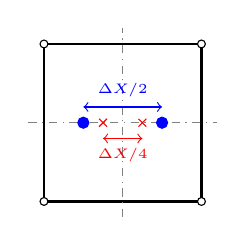
\begin{tikzpicture}[scale=1.]
    \draw[black,thick] (-1.,-1.) rectangle (1.,1.);
    \draw[black!50,dashdotted] (-1.2,0.) -- (1.2,0.0);\draw[black!50,dashdotted] (.0,-1.2) -- (0.,1.2);
    %% nodes
    \fill[white] (-1,-1) circle (0.05);\draw (-1,-1) circle (0.05);
    \fill[white] (1.,-1) circle (0.05);\draw (1,-1) circle (0.05);
    \fill[white] (1,1) circle (0.05);\draw (1,1) circle (0.05);
    \fill[white] (-1.,1) circle (0.05);\draw (-1,1) circle (0.05);
    %% particles
    \draw[Blue,mark=*] plot coordinates {(-0.5,0.)};
    \draw[Blue,mark=*] plot coordinates {(0.5,0.)};
    \draw[Blue,<->] (-0.5,0.2) -- (0.5,0.2) node [midway,above] {\tiny $\Delta X/2$};
    \draw[Red,mark=x] plot coordinates {(-0.25,0.)};
    \draw[Red,mark=x] plot coordinates {(0.25,0.)};
    \draw[Red,<->] (-0.25,-0.2) -- (0.25,-0.2) node [midway,below] {\tiny $\Delta X/4$};
  \end{tikzpicture}  & 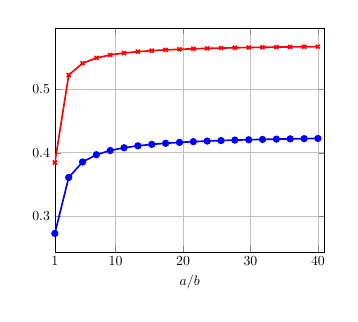
\begin{tikzpicture}[scale=0.5]
\begin{axis}[xlabel=$a/b$,ymajorgrids=true,xmajorgrids=true,xmin=1,xmax=41,xtick={1,10,20,30,40}]
%%%%%%%%%%% NATURAL CONFIGURATION
\addplot[Blue,mark=*,very thick] coordinates {(1.0,0.272727272727) (3.05263157895,0.360995850622) (5.10526315789,0.385430463576) (7.15789473684,0.396887159533) (9.21052631579,0.403535741737) (11.2631578947,0.407878017789) (13.3157894737,0.410936654034) (15.3684210526,0.41320754717) (17.4210526316,0.414960300878) (19.4736842105,0.416354088522) (21.5263157895,0.417488941817) (23.5789473684,0.418430884184) (25.6315789474,0.419225251076) (27.6842105263,0.419904204364) (29.7368421053,0.420491193252) (31.7894736842,0.421003717472) (33.8421052632,0.421455101595) (35.8947368421,0.421855670103) (37.9473684211,0.42221354675) (40.0,0.422535211268) };
%%%%%%%%%%% MODIFIED CONFIGURATION
\addplot[Red,mark=x,very thick] coordinates {(1.0,0.384615384615) (3.05263157895,0.522522522523) (5.10526315789,0.541143654114) (7.15789473684,0.549494949495) (9.21052631579,0.55423594616) (11.2631578947,0.557291666667) (13.3157894737,0.559425096739) (15.3684210526,0.560999039385) (17.4210526316,0.562208067941) (19.4736842105,0.563165905632) (21.5263157895,0.56394346777) (23.5789473684,0.564587271582) (25.6315789474,0.565129097766) (27.6842105263,0.565591397849) (29.7368421053,0.565990483346) (31.7894736842,0.566338490389) (33.8421052632,0.566644635382) (35.8947368421,0.566916043225) (37.9473684211,0.567158308751) (40.0,0.567375886525) };
\end{axis}
\end{tikzpicture}
%%% Local Variables:
%%% mode: latex
%%% TeX-master: "../../mainManuscript"
%%% End:
 & 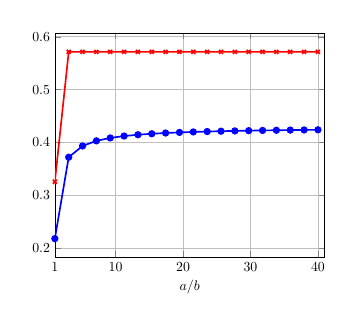
\begin{tikzpicture}[scale=0.5]
\begin{axis}[xlabel=$a/b$,ymajorgrids=true,xmajorgrids=true,xmin=1,xmax=41,xtick={1,10,20,30,40}]
%%%%%%%%%%% NATURAL CONFIGURATION
\addplot[Blue,mark=*,very thick] coordinates {(1.0,0.217751156849) (3.05263157895,0.371899923259) (5.10526315789,0.393212462993) (7.15789473684,0.402887246166) (9.21052631579,0.40840759179) (11.2631578947,0.411975544) (13.3157894737,0.414470966386) (15.3684210526,0.416314181564) (17.4210526316,0.417731290591) (19.4736842105,0.418854723411) (21.5263157895,0.419767189778) (23.5789473684,0.420523008979) (25.6315789474,0.421159327636) (27.6842105263,0.421702408465) (29.7368421053,0.422171344199) (31.7894736842,0.422580347983) (33.8421052632,0.422940218545) (35.8947368421,0.423259307375) (37.9473684211,0.423544174777) (40.0,0.423800045624) };
%%%%%%%%%%% MODIFIED CONFIGURATION
\addplot[Red,mark=x,very thick] coordinates {(1.0,0.325412497399) (3.05263157895,0.571428571428) (5.10526315789,0.571428571429) (7.15789473684,0.571428571429) (9.21052631579,0.57142857143) (11.2631578947,0.571428571429) (13.3157894737,0.571428571429) (15.3684210526,0.571428571429) (17.4210526316,0.571428571429) (19.4736842105,0.571428571429) (21.5263157895,0.571428571429) (23.5789473684,0.571428571429) (25.6315789474,0.571428571429) (27.6842105263,0.571428571429) (29.7368421053,0.571428571429) (31.7894736842,0.571428571429) (33.8421052632,0.571428571429) (35.8947368421,0.571428571429) (37.9473684211,0.571428571429) (40.0,0.571428571429) };
\end{axis}
\end{tikzpicture}
%%% Local Variables:
%%% mode: latex
%%% TeX-master: "../../mainManuscript"
%%% End:
&\\ [3.25cm]%%% SOLUTION
  \hline
  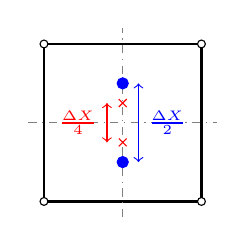
\begin{tikzpicture}[scale=1.]
    \draw[black,thick] (-1.,-1.) rectangle (1.,1.);
    \draw[black!50,dashdotted] (-1.2,0.) -- (1.2,0.0);\draw[black!50,dashdotted] (.0,-1.2) -- (0.,1.2);
    %% nodes
    \fill[white] (-1,-1) circle (0.05);\draw (-1,-1) circle (0.05);
    \fill[white] (1.,-1) circle (0.05);\draw (1,-1) circle (0.05);
    \fill[white] (1,1) circle (0.05);\draw (1,1) circle (0.05);
    \fill[white] (-1.,1) circle (0.05);\draw (-1,1) circle (0.05);
    %% particles
    \draw[Blue,mark=*] plot coordinates {(-0.,-0.5)};
    \draw[Blue,mark=*] plot coordinates {(0.,0.5)};
    \draw[Blue,<->] (0.2,-0.5) -- (0.2,0.5) node [midway,right] {\scriptsize $\frac{\Delta X}{2}$};
    \draw[Red,mark=x] plot coordinates {(0.,-0.25)};
    \draw[Red,mark=x] plot coordinates {(0.,0.25)};
    \draw[Red,<->] (-0.2,-0.25) -- (-0.2,0.25) node [midway,left] {\scriptsize $\frac{\Delta X}{4}$};
  \end{tikzpicture}  & 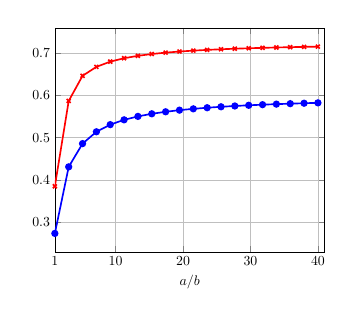
\begin{tikzpicture}[scale=0.5]
\begin{axis}[xlabel=$a/b$,ymajorgrids=true,xmajorgrids=true,xmin=1,xmax=41,xtick={1,10,20,30,40}]
%%%%%%%%%%% NATURAL CONFIGURATION
\addplot[Blue,mark=*,very thick] coordinates {(1.0,0.272727272727) (3.05263157895,0.430693069307) (5.10526315789,0.485809682805) (7.15789473684,0.513853904282) (9.21052631579,0.530839231547) (11.2631578947,0.54222972973) (13.3157894737,0.550398839739) (15.3684210526,0.556543837357) (17.4210526316,0.561334087055) (19.4736842105,0.56517311609) (21.5263157895,0.568318666049) (23.5789473684,0.570943075616) (25.6315789474,0.57316594743) (27.6842105263,0.575072886297) (29.7368421053,0.576726777816) (31.7894736842,0.578174856414) (33.8421052632,0.579453289276) (35.8947368421,0.580590238365) (37.9473684211,0.581607959129) (40.0,0.582524271845) };
%%%%%%%%%%% MODIFIED CONFIGURATION
\addplot[Red,mark=x,very thick] coordinates {(1.0,0.384615384615) (3.05263157895,0.587044534413) (5.10526315789,0.646666666667) (7.15789473684,0.667894413751) (9.21052631579,0.680272108844) (11.2631578947,0.688379573784) (13.3157894737,0.694101508916) (15.3684210526,0.698355754858) (17.4210526316,0.70164281929) (19.4736842105,0.704258862717) (21.5263157895,0.706390328152) (23.5789473684,0.7081604426) (25.6315789474,0.709653916211) (27.6842105263,0.71093090049) (29.7368421053,0.712035286704) (31.7894736842,0.712999852442) (33.8421052632,0.713849569803) (35.8947368421,0.714603798297) (37.9473684211,0.715277777778) (40.0,0.715883668904) };
\end{axis}
\end{tikzpicture}
%%% Local Variables:
%%% mode: latex
%%% TeX-master: "../../mainManuscript"
%%% End:
 & 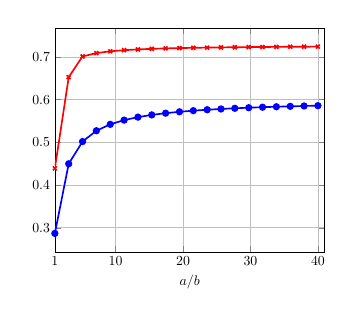
\begin{tikzpicture}[scale=0.5]
\begin{axis}[xlabel=$a/b$,ymajorgrids=true,xmajorgrids=true,xmin=1,xmax=41,xtick={1,10,20,30,40}]
%%%%%%%%%%% NATURAL CONFIGURATION
\addplot[Blue,mark=*,very thick] coordinates {(1.0,0.286705918022) (3.05263157895,0.449716071021) (5.10526315789,0.501782746472) (7.15789473684,0.527153462699) (9.21052631579,0.54213191771) (11.2631578947,0.552009414669) (13.3157894737,0.559009934788) (15.3684210526,0.564229666081) (17.4210526316,0.568271008297) (19.4736842105,0.571492328044) (21.5263157895,0.574120115076) (23.5789473684,0.576304512257) (25.6315789474,0.578148974898) (27.6842105263,0.579727104075) (29.7368421053,0.581092688356) (31.7894736842,0.58228594869) (33.8421052632,0.583337561737) (35.8947368421,0.584271331895) (37.9473684211,0.585106013388) (40.0,0.585856581891) };
%%%%%%%%%%% MODIFIED CONFIGURATION
\addplot[Red,mark=x,very thick] coordinates {(1.0,0.438891399031) (3.05263157895,0.652556925298) (5.10526315789,0.701154248564) (7.15789473684,0.708927502176) (9.21052631579,0.713138668165) (11.2631578947,0.715778473448) (13.3157894737,0.717587786989) (15.3684210526,0.718905133196) (17.4210526316,0.719907103779) (19.4736842105,0.720694821913) (21.5263157895,0.721330359644) (23.5789473684,0.721853926318) (25.6315789474,0.722292713971) (27.6842105263,0.722665770137) (29.7368421053,0.722986834444) (31.7894736842,0.723266066974) (33.8421052632,0.723511142614) (35.8947368421,0.72372796708) (37.9473684211,0.72392115889) (40.0,0.724094381918) };
\end{axis}
\end{tikzpicture}
%%% Local Variables:
%%% mode: latex
%%% TeX-master: "../../mainManuscript"
%%% End:
& \\ [3.25cm] %%% SOLUTION
  \hline
\end{tabular}

%%% Local Variables: 
%%% mode: latex
%%% TeX-master: "../../mainManuscript"
%%% End:
  \caption{Values of critical Courant number $s_1\frac{\Delta t}{\Delta x}$ for two-dimensional DGMPM scheme using either DCU or CTU with respect to the locations of the two material points lying in every cells, as a function of the speeds ratio $s_1/s_2$.}
  \label{tab:2DCFL_comparison_2ppc}
\end{table}
First, the results of table \ref{tab:2DCFL_comparison_2ppc} show that the CFL number exhibits a non-linear dependence on the speed ratio $s_1/s_2$, which asymptotically approach some value depending on the particles distribution.
The configuration in which the particles are regularly spaced in the grid is of particular interest.
Indeed, this discretization is equivalent to the vertical repetition of the natural configuration for two particles per cell studied in section \ref{sec:1d_stab}.
As a result, the one-dimensional result for Euler discretization $CFL \approx 0.43$ should be recovered for $s_1 \gg s_2$.
This value is depicted with black dashed lines in the plots of first row in table \ref{tab:2DCFL_comparison_2ppc}.
It is thus seen that the one-dimensional value of the Courant number corresponds to the asymptotic limit for two-dimensional problems as $s_1/s_2 \rightarrow \infty$.
% In particular, the configuration drawn in blue plus signs in the first row is equivalent, for $s_1 \gg s_2$, to the one-dimensional natural configuration for two particles per cell studied in section \ref{sec:1d_stab}.
% As a result, the CFL number tends to the value $0.43$ determined in one space dimension as $s_1/s_2 \rightarrow \infty$, which is depicted with the black dashed lines in the CFL curves.

Next, the spacing between particles is reduced while keeping the symmetry with respect to cells centers.
It is then seen that, as for one-dimensional case, the critical Courant number increases for both DCU and CTU approaches.
%Second, we see that a reduction of spacing between particles ensuring symmetry between them with respect to cells centers, as for one-dimensional case, yields an increase in the critical Courant number for both DCU and CTU approaches. 
Third, whether particles lie on the horizontal axis or the vertical axis of cells has a great influence on the critical Courant number one can expect.
Hence, the configurations of the second row of table \ref{tab:2DCFL_comparison_2ppc} yield higher CFL numbers for given speed ratios.
It then appears that in order to improve the stability of the scheme, one must use a lower number of material points in the direction of the dominating wave speed than in the perpendicular one.
For a Cartesian distribution of particles $N_p^x \times N_p^y$ this corresponds to $N_p^y > N_p^x$ if $s_1>s_2$, and $N_p^x > N_p^y$ if $s_2>s_1$.
At last, it is worth noticing that the improvement brought by the CTU is much less significant than in the case of one single particle-per-cell discretization for which the Courant number can be set to one according to equations \eqref{eq:2D_CFL_DCU} and \eqref{eq:2D_CFL_CTU}.

%% 4ppc
\begin{table}[h!]
  \centering
  \begin{tabular}[ht]{M{2.5cm}M{5.cm}M{5.cm}N}
  %\setlength\extrarowheight{2.5pt}
  \hline
  Particles in cells & \multicolumn{2}{c}{Critical Courant number $\frac{a\Delta t}{\Delta X}(a/b)$}  & \\[0.5cm]
   &  DCU & CTU & \\
%   & & \multicolumn{2}{c}{$a/b=1$} & \multicolumn{2}{c}{$a/b=10$} & \multicolumn{2}{c}{$a/b=1$} & \multicolumn{2}{c}{$a/b=10$}\\
   % Particles & Position of particles in cell $c$ &  \multicolumn{2}{c}{DCU} & \multicolumn{2}{c}{DCU} \\
  \hline
  \hline
  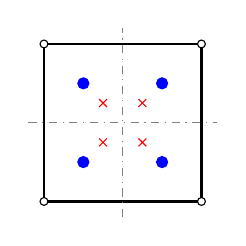
\begin{tikzpicture}[scale=1.]
    \draw[black,thick] (-1.,-1.) rectangle (1.,1.);
    \draw[black!50,dashdotted] (-1.2,0.) -- (1.2,0.0);\draw[black!50,dashdotted] (.0,-1.2) -- (0.,1.2);
    %% nodes
    \fill[white] (-1,-1) circle (0.05);\draw (-1,-1) circle (0.05);
    \fill[white] (1.,-1) circle (0.05);\draw (1,-1) circle (0.05);
    \fill[white] (1,1) circle (0.05);\draw (1,1) circle (0.05);
    \fill[white] (-1.,1) circle (0.05);\draw (-1,1) circle (0.05);
    %% particles
    \draw[Blue,mark=*] plot coordinates {(-0.5,-0.5)};
    \draw[Blue,mark=*] plot coordinates {(0.5,0.5)};
    \draw[Blue,mark=*] plot coordinates {(-0.5,0.5)};
    \draw[Blue,mark=*] plot coordinates {(0.5,-0.5)};
    %\draw[Blue,|-|] (0.5,-0.5) -- (0.5,0.5) node [midway,right] {\scriptsize $\frac{\Delta X}{2}$};
    \draw[Red,mark=x] plot coordinates {(-0.25,-0.25)};
    \draw[Red,mark=x] plot coordinates {(0.25,0.25)};
    \draw[Red,mark=x] plot coordinates {(-0.25,0.25)};
    \draw[Red,mark=x] plot coordinates {(0.25,-0.25)};
    %\draw[Red,|-|] (-0.25,-0.25) -- (-0.25,0.25) node [midway,left] {\scriptsize $\frac{\Delta X}{4}$};
  \end{tikzpicture} & 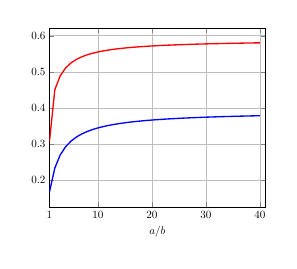
\begin{tikzpicture}[scale=0.4]
\begin{axis}[xlabel=$a/b$,ymajorgrids=true,xmajorgrids=true,xmin=1,xmax=41,xtick={1,10,20,30,40}]
%%%%%%%%%%% NATURAL CONFIGURATION
\addplot[Blue,very thick] coordinates {(1.0,0.166666666667) (2.0,0.233766233766) (3.0,0.27) (4.0,0.292682926829) (5.0,0.308219178082) (6.0,0.319526627219) (7.0,0.328125) (8.0,0.33488372093) (9.0,0.340336134454) (10.0,0.344827586207) (11.0,0.348591549296) (12.0,0.351791530945) (13.0,0.354545454545) (14.0,0.356940509915) (15.0,0.359042553191) (16.0,0.360902255639) (17.0,0.362559241706) (18.0,0.36404494382) (19.0,0.365384615385) (20.0,0.366598778004) (21.0,0.367704280156) (22.0,0.368715083799) (23.0,0.369642857143) (24.0,0.370497427101) (25.0,0.371287128713) (26.0,0.372019077901) (27.0,0.372699386503) (28.0,0.373333333333) (29.0,0.373925501433) (30.0,0.374479889043) (31.0,0.375) (32.0,0.375488917862) (33.0,0.375949367089) (34.0,0.376383763838) (35.0,0.376794258373) (36.0,0.377182770664) (37.0,0.377551020408) (38.0,0.377900552486) (39.0,0.378232758621) (40.0,0.378548895899) };
%%%%%%%%%%% MODIFIED CONFIGURATION
\addplot[Red,very thick] coordinates {(1.0,0.30612244898) (2.0,0.450574712644) (3.0,0.488913525499) (4.0,0.510638297872) (5.0,0.524625267666) (6.0,0.534383520145) (7.0,0.541578947368) (8.0,0.547103977669) (9.0,0.551479783243) (10.0,0.555031149707) (11.0,0.557971014493) (12.0,0.560444797458) (13.0,0.562555195761) (14.0,0.564376799671) (15.0,0.565965092402) (16.0,0.567362199976) (17.0,0.568600682594) (18.0,0.569706103994) (19.0,0.570698814875) (20.0,0.571595217265) (21.0,0.572408677916) (22.0,0.57315019938) (23.0,0.57382892057) (24.0,0.574452495319) (25.0,0.575027382256) (26.0,0.575559069347) (27.0,0.576052249637) (28.0,0.576510960151) (29.0,0.576938692651) (30.0,0.577338482686) (31.0,0.577712981744) (32.0,0.578064516129) (33.0,0.578395135328) (34.0,0.578706652) (35.0,0.579000675219) (36.0,0.579278638279) (37.0,0.579541822056) (38.0,0.579791374747) (39.0,0.580028328612) (40.0,0.58025361425) };
\end{axis}
\end{tikzpicture}
%%% Local Variables:
%%% mode: latex
%%% TeX-master: "../../mainManuscript"
%%% End:
 & 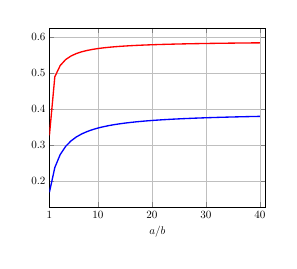
\begin{tikzpicture}[scale=0.4]
\begin{axis}[xlabel=$a/b$,ymajorgrids=true,xmajorgrids=true,xmin=1,xmax=41,xtick={1,10,20,30,40}]
%%%%%%%%%%% NATURAL CONFIGURATION
\addplot[Blue,very thick] coordinates {(1.0,0.167891991267) (2.0,0.236676134687) (3.0,0.272980739363) (4.0,0.295523052838) (5.0,0.31086679909) (6.0,0.321980387453) (7.0,0.330399242911) (8.0,0.336996589796) (9.0,0.342305428681) (10.0,0.346669420492) (11.0,0.350320058356) (12.0,0.353418957124) (13.0,0.356082359353) (14.0,0.358396007915) (15.0,0.360424530234) (16.0,0.362217559503) (17.0,0.363813843724) (18.0,0.36524407401) (19.0,0.366532874772) (20.0,0.367700231858) (21.0,0.368762535467) (22.0,0.369733353839) (23.0,0.370624015434) (24.0,0.371444052722) (25.0,0.372201544487) (26.0,0.372903382721) (27.0,0.373555482814) (28.0,0.374162950599) (29.0,0.374730216246) (30.0,0.375261142441) (31.0,0.375759112422) (32.0,0.376227102125) (33.0,0.376667739677) (34.0,0.377083354767) (35.0,0.377476019835) (36.0,0.37784758462) (37.0,0.378199705293) (38.0,0.378533869127) (39.0,0.378851415496) (40.0,0.379153553806) };
%%%%%%%%%%% MODIFIED CONFIGURATION
\addplot[Red,very thick] coordinates {(1.0,0.326304188278) (2.0,0.489325348197) (3.0,0.520649204857) (4.0,0.537092735424) (5.0,0.547194071957) (6.0,0.554021734434) (7.0,0.558942755592) (8.0,0.56265696686) (9.0,0.565559375666) (10.0,0.567889697418) (11.0,0.56980178835) (12.0,0.571398904651) (13.0,0.572752913461) (14.0,0.573915372853) (15.0,0.57492422974) (16.0,0.575808031925) (17.0,0.57658866765) (18.0,0.577283199978) (19.0,0.577905126649) (20.0,0.578465264862) (21.0,0.578972385091) (22.0,0.579433673213) (23.0,0.579855072848) (24.0,0.580241542647) (25.0,0.580597252178) (26.0,0.580925732862) (27.0,0.581229995544) (28.0,0.581512622996) (29.0,0.58177584338) (30.0,0.582021589074) (31.0,0.58225154418) (32.0,0.582467183146) (33.0,0.58266980241) (34.0,0.582860546471) (35.0,0.583040429512) (36.0,0.583210353437) (37.0,0.583371122983) (38.0,0.583523458467) (39.0,0.583668006571) (40.0,0.583805349515) };
\end{axis}
\end{tikzpicture}
%%% Local Variables:
%%% mode: latex
%%% TeX-master: "../../mainManuscript"
%%% End:
& \\ [3.25cm]
  %%%%%%%%%%%%%%%%%%%%%%%%%%%%%%%%%%%%%%%
  %%%%%%%%%%%%%%%%%%%%%%%%%%%%%%%%%%%%%%% 
  \hline % Shifted left // Shifted right
  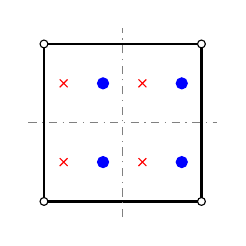
\begin{tikzpicture}[scale=1.]
    \draw[black,thick] (-1.,-1.) rectangle (1.,1.);
    \draw[black!50,dashdotted] (-1.2,0.) -- (1.2,0.0);\draw[black!50,dashdotted] (.0,-1.2) -- (0.,1.2);
    %% nodes
    \fill[white] (-1,-1) circle (0.05);\draw (-1,-1) circle (0.05);
    \fill[white] (1.,-1) circle (0.05);\draw (1,-1) circle (0.05);
    \fill[white] (1,1) circle (0.05);\draw (1,1) circle (0.05);
    \fill[white] (-1.,1) circle (0.05);\draw (-1,1) circle (0.05);
    %% particles
    \draw[Blue,mark=*] plot coordinates {(-0.5+0.25,-0.5)};
    \draw[Blue,mark=*] plot coordinates {(0.5+0.25,0.5)};
    \draw[Blue,mark=*] plot coordinates {(-0.5+0.25,0.5)};
    \draw[Blue,mark=*] plot coordinates {(0.5+0.25,-0.5)};
    \draw[Red,mark=x] plot coordinates {(-0.5-0.25,-0.5)};
    \draw[Red,mark=x] plot coordinates {(0.5-0.25,0.5)};
    \draw[Red,mark=x] plot coordinates {(-0.5-0.25,0.5)};
    \draw[Red,mark=x] plot coordinates {(0.5-0.25,-0.5)};
  \end{tikzpicture}  & 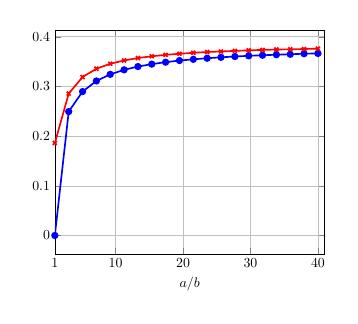
\begin{tikzpicture}[scale=0.5]
\begin{axis}[xlabel=$a/b$,ymajorgrids=true,xmajorgrids=true,xmin=1,xmax=41,xtick={1,10,20,30,40}]
%%%%%%%%%%% NATURAL CONFIGURATION
\addplot[Blue,mark=*,very thick] coordinates {(1.0,1.0000100001e-05) (3.05263157895,0.249310914162) (5.10526315789,0.28957342205) (7.15789473684,0.311013636452) (9.21052631579,0.324305874638) (11.2631578947,0.333392807612) (13.3157894737,0.339955504818) (15.3684210526,0.344870817129) (17.4210526316,0.348772961414) (19.4736842105,0.352087731404) (21.5263157895,0.354541966472) (23.5789473684,0.356753041215) (25.6315789474,0.358589375367) (27.6842105263,0.360175180699) (29.7368421053,0.361603616036) (31.7894736842,0.362721521952) (33.8421052632,0.363806269642) (35.8947368421,0.364694173258) (37.9473684211,0.365816289742) (40.0,0.366403664037) };
%%%%%%%%%%% MODIFIED CONFIGURATION
\addplot[Red,mark=x,very thick] coordinates {(1.0,0.186161861619) (3.05263157895,0.285515486734) (5.10526315789,0.318877925621) (7.15789473684,0.335565460918) (9.21052631579,0.345582403192) (11.2631578947,0.352315102098) (13.3157894737,0.357133045015) (15.3684210526,0.36070044911) (17.4210526316,0.363581004231) (19.4736842105,0.365719446668) (21.5263157895,0.367673150416) (23.5789473684,0.36925000829) (25.6315789474,0.37038001959) (27.6842105263,0.371525820521) (29.7368421053,0.372606357643) (31.7894736842,0.37353005109) (33.8421052632,0.374297427185) (35.8947368421,0.37474480008) (37.9473684211,0.375303226716) (40.0,0.376003760038) };
\end{axis}
\end{tikzpicture}
%%% Local Variables:
%%% mode: latex
%%% TeX-master: "../../mainManuscript"
%%% End:
 &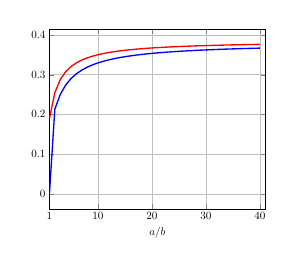
\begin{tikzpicture}[scale=0.4]
\begin{axis}[xlabel=$a/b$,ymajorgrids=true,xmajorgrids=true,xmin=1,xmax=41,xtick={1,10,20,30,40}]
%%%%%%%%%%% NATURAL CONFIGURATION
\addplot[Blue,very thick] coordinates {(1.0,-1.59364188514e-12) (2.0,0.212857320897) (3.0,0.249893924351) (4.0,0.27360416432) (5.0,0.290070593852) (6.0,0.30216822431) (7.0,0.311430129824) (8.0,0.318747857117) (9.0,0.324674954147) (10.0,0.329573175966) (11.0,0.333688883167) (12.0,0.337195633388) (13.0,0.340219213023) (14.0,0.342853009248) (15.0,0.345167807082) (16.0,0.347218235209) (17.0,0.349047125479) (18.0,0.350688533417) (19.0,0.352169876071) (20.0,0.3535134741) (21.0,0.354737683146) (22.0,0.355857736689) (23.0,0.356886382692) (24.0,0.357834370589) (25.0,0.358710828109) (26.0,0.359523555947) (27.0,0.360279260443) (28.0,0.360983738964) (29.0,0.361642028851) (30.0,0.362258527996) (31.0,0.362837093184) (32.0,0.36338112082) (33.0,0.363893613627) (34.0,0.364377236081) (35.0,0.364834360724) (36.0,0.365267107082) (37.0,0.365677374516) (38.0,0.36606687008) (39.0,0.366437132262) (40.0,0.366789551283) };
%%%%%%%%%%% MODIFIED CONFIGURATION
\addplot[Red,very thick] coordinates {(1.0,0.18887015067) (2.0,0.254459520239) (3.0,0.287403904864) (4.0,0.307169534548) (5.0,0.320334758075) (6.0,0.329729082668) (7.0,0.336768311765) (8.0,0.342238808871) (9.0,0.346612107914) (10.0,0.350188061313) (11.0,0.353166425063) (12.0,0.355685394958) (13.0,0.357843617559) (14.0,0.359713389803) (15.0,0.361348904135) (16.0,0.362791580609) (17.0,0.364073619671) (18.0,0.36522043174) (19.0,0.366252337065) (20.0,0.367185779335) (21.0,0.368034207917) (22.0,0.368808729666) (23.0,0.369518597597) (24.0,0.370171582133) (25.0,0.370774256583) (26.0,0.371332219112) (27.0,0.371850267081) (28.0,0.372332535292) (29.0,0.372782606539) (30.0,0.373203600747) (31.0,0.373598247379) (32.0,0.373968944663) (33.0,0.374317808349) (34.0,0.374646712123) (35.0,0.374957321245) (36.0,0.375251120754) (37.0,0.375529439201) (38.0,0.375793468735) (39.0,0.376044282167) (40.0,0.376282847537) };
\end{axis}
\end{tikzpicture}
%%% Local Variables:
%%% mode: latex
%%% TeX-master: "../../mainManuscript"
%%% End:
& \\ [3.25cm]
  %%%%%%%%%%%%%%%%%%%%%%%%%%%%%%%%%%%%%
  %%%%%%%%%%%%%%%%%%%%%%%%%%%%%%%%%%%%%
  \hline % Shifted above // Shifted below
  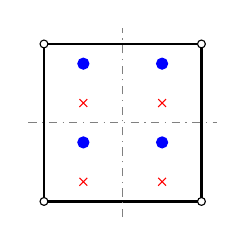
\begin{tikzpicture}[scale=1.]
    \draw[black,thick] (-1.,-1.) rectangle (1.,1.);
    \draw[black!50,dashdotted] (-1.2,0.) -- (1.2,0.0);\draw[black!50,dashdotted] (.0,-1.2) -- (0.,1.2);
    %% nodes
    \fill[white] (-1,-1) circle (0.05);\draw (-1,-1) circle (0.05);
    \fill[white] (1.,-1) circle (0.05);\draw (1,-1) circle (0.05);
    \fill[white] (1,1) circle (0.05);\draw (1,1) circle (0.05);
    \fill[white] (-1.,1) circle (0.05);\draw (-1,1) circle (0.05);
    %% particles
    \draw[Blue,mark=*] plot coordinates {(-0.5,-0.5+0.25)};
    \draw[Blue,mark=*] plot coordinates {(0.5,0.5+0.25)};
    \draw[Blue,mark=*] plot coordinates {(-0.5,0.5+0.25)};
    \draw[Blue,mark=*] plot coordinates {(0.5,-0.5+0.25)};
    \draw[Red,mark=x] plot coordinates {(-0.5,-0.5-0.25)};
    \draw[Red,mark=x] plot coordinates {(0.5,0.5-0.25)};
    \draw[Red,mark=x] plot coordinates {(-0.5,0.5-0.25)};
    \draw[Red,mark=x] plot coordinates {(0.5,-0.5-0.25)};
  \end{tikzpicture}& 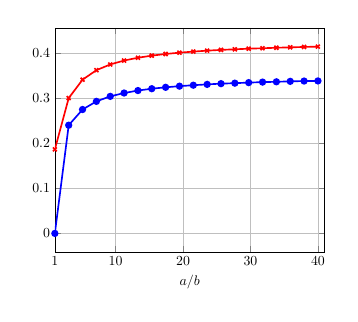
\begin{tikzpicture}[scale=0.5]
\begin{axis}[xlabel=$a/b$,ymajorgrids=true,xmajorgrids=true,xmin=1,xmax=41,xtick={1,10,20,30,40}]
%%%%%%%%%%% NATURAL CONFIGURATION
\addplot[Blue,mark=*,very thick] coordinates {(1.0,1.0000100001e-05) (3.05263157895,0.239878188256) (5.10526315789,0.274614851412) (7.15789473684,0.292689242682) (9.21052631579,0.303766195557) (11.2631578947,0.311204164673) (13.3157894737,0.316652640211) (15.3684210526,0.32074215479) (17.4210526316,0.323860607027) (19.4736842105,0.326382211191) (21.5263157895,0.328494863896) (23.5789473684,0.330344356075) (25.6315789474,0.331932266691) (27.6842105263,0.333044383075) (29.7368421053,0.334245447718) (31.7894736842,0.335382301191) (33.8421052632,0.336055465818) (35.8947368421,0.337054949497) (37.9473684211,0.337734956297) (40.0,0.338003380034) };
%%%%%%%%%%% MODIFIED CONFIGURATION
\addplot[Red,mark=x,very thick] coordinates {(1.0,0.186161861619) (3.05263157895,0.299954578493) (5.10526315789,0.340728670445) (7.15789473684,0.361763617636) (9.21052631579,0.374503745037) (11.2631578947,0.383176463344) (13.3157894737,0.389357577786) (15.3684210526,0.394050256292) (17.4210526316,0.397726608845) (19.4736842105,0.400577689987) (21.5263157895,0.402976661346) (23.5789473684,0.405090366693) (25.6315789474,0.406777225667) (27.6842105263,0.408069343851) (29.7368421053,0.409480410594) (31.7894736842,0.410406209325) (33.8421052632,0.411524115241) (35.8947368421,0.412434650662) (37.9473684211,0.413250974615) (40.0,0.414004140041) };
\end{axis}
\end{tikzpicture}
%%% Local Variables:
%%% mode: latex
%%% TeX-master: "../../mainManuscript"
%%% End:
 &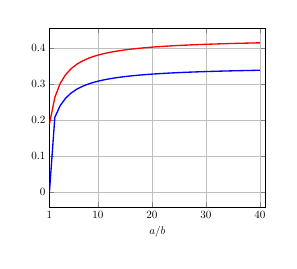
\begin{tikzpicture}[scale=0.4]
\begin{axis}[xlabel=$a/b$,ymajorgrids=true,xmajorgrids=true,xmin=1,xmax=41,xtick={1,10,20,30,40}]
%%%%%%%%%%% NATURAL CONFIGURATION
\addplot[Blue,very thick] coordinates {(1.0,-6.54115650537e-13) (2.0,0.207631685065) (3.0,0.240430029398) (4.0,0.26096289659) (5.0,0.275016910974) (6.0,0.285237324443) (7.0,0.293003101823) (8.0,0.299103117316) (9.0,0.304021109389) (10.0,0.308070133656) (11.0,0.311461709667) (12.0,0.314343883947) (13.0,0.316823369995) (14.0,0.318979027962) (15.0,0.320870393341) (16.0,0.322543253386) (17.0,0.324033398269) (18.0,0.325369207815) (19.0,0.326573474704) (20.0,0.327664714709) (21.0,0.328658124781) (22.0,0.329566294666) (23.0,0.330399742969) (24.0,0.331167326188) (25.0,0.331876554506) (26.0,0.332533838231) (27.0,0.33314468201) (28.0,0.333713839307) (29.0,0.334245436298) (30.0,0.334743072039) (31.0,0.335209900028) (32.0,0.335648695078) (33.0,0.336061908505) (34.0,0.336451713928) (35.0,0.336820045512) (36.0,0.337168630053) (37.0,0.337499014044) (38.0,0.337812586608) (39.0,0.33811059902) (40.0,0.338394181387) };
%%%%%%%%%%% MODIFIED CONFIGURATION
\addplot[Red,very thick] coordinates {(1.0,0.18887015067) (2.0,0.262956392078) (3.0,0.302076047328) (4.0,0.32618849157) (5.0,0.342522128096) (6.0,0.354312580524) (7.0,0.363221663933) (8.0,0.370189579051) (9.0,0.375787926093) (10.0,0.380384094421) (11.0,0.384224929247) (12.0,0.387482399219) (13.0,0.390279973956) (14.0,0.392708588922) (15.0,0.394836695539) (16.0,0.396716803678) (17.0,0.398389865869) (18.0,0.399888290415) (19.0,0.401238058753) (20.0,0.402460243029) (21.0,0.403572113124) (22.0,0.404587957102) (23.0,0.405519698035) (24.0,0.406377363812) (25.0,0.407169449254) (26.0,0.407903198264) (27.0,0.408584825881) (28.0,0.409219694664) (29.0,0.409812455992) (30.0,0.410367164166) (31.0,0.41088736923) (32.0,0.411376192992) (33.0,0.411836391706) (34.0,0.412270408049) (35.0,0.412680414481) (36.0,0.413068349603) (37.0,0.413435948794) (38.0,0.413784770166) (39.0,0.414116216626) (40.0,0.414431554738) };
\end{axis}
\end{tikzpicture}
%%% Local Variables:
%%% mode: latex
%%% TeX-master: "../../mainManuscript"
%%% End:
& \\ [3.25cm]
  %\begin{minipage}{0.85\textwidth}\lipsum[1]\end{minipage}
  \hline
\end{tabular}

%%% Local Variables: 
%%% mode: latex
%%% TeX-master: "../../mainManuscript"
%%% End:
  \caption{Values of critical Courant number $s_1\frac{\Delta t}{\Delta x}$ for two-dimensional DGMPM scheme using either DCU or CTU with respect to the material points distribution, as a function of the speeds ratio $s_1/s_2$.}
  \label{tab:2DCFL_comparison_4ppc}
\end{table}
We now move on to cases for which grid cells each contains four material points, by considering a square shaped distribution of particles in every elements. %which centers coincide with cells centroids.
This square distribution is such that the particles are initially regularly spaced in horizontal and vertical directions, and is deformed so that the following situations occur:
\begin{itemize}
\item the particles are displaced while keeping the center of the square of material points on the cells centroids.
  Three configurations are then depicted in the first row of table \ref{tab:2DCFL_comparison_4ppc}.
\item the square of particles is translated horizontally without distortion as depicted in the second row of the table.
\item the square of particles is translated vertically without distortion (third row of the table).
\end{itemize}

%In the first row of table \ref{tab:2DCFL_comparison_4ppc}, the particles are displaced while keeping the center of the square of material points on the cells centroids.
%On the other hand, the second and third rows of the table investigate of a simple translation of the square pattern in the elements without distortion.  
% This pattern can be contracted or simply translated without change of shape as depicted in the first column of table \ref{tab:2DCFL_comparison_4ppc}.
%Several configurations are gathered in each row of the table and are distinguished by using different colors and markers.

First, we see in the first row of table \ref{tab:2DCFL_comparison_4ppc} that the contraction of the square shaped distribution of particles yields an improvement of the critical CFL number.
These observations are similar to those made for one-dimensional problems, especially for the configuration in which the particles coincide with nodes that leads to a vanishing Courant number (see green curves with star marks).
On the other hand, the increase in CFL number enabled by the use of the CTU approach is again less important that in the case of one particle per cell.

Second, the last two rows of table \ref{tab:2DCFL_comparison_4ppc} show that the translation of the square of particle inside elements does not have great influence on the evolution of Courant's number with respect to the speed ratio.
Nonetheless, it can be seen that a slight increase in CFL number results from an upwind displacement of particles, as observed for the one-dimensional scheme.
At last, the curves corresponding to DCU and CTU do not exhibit significant differences, meaning that the CTU seems to be mainly efficient for the one particle per cell discretization.
%Finally, it can be seen from the two last rows of table \ref{tab:2DCFL_comparison_4ppc} that the translation of the square of particle inside elements does not have great influence on the evolution of Courant's number with respect to the speed ratio. 


%% 9ppc
Similar distributions of nine particles with square shapes are now looked at.
Analogously to the four particles per cell discretization, the square pattern is either distorted or translated inside the cells and the resulting CFL numbers are gathered in table \ref{tab:2DCFL_comparison_9ppc}.
\begin{table}[h!]
  \centering
  \input{tabular/2DCFL_comparison_9ppc}
  \caption{Values of critical Courant number $s_1\frac{\Delta t}{\Delta x}$ for two-dimensional DGMPM scheme using either DCU or CTU with respect to the material points distribution, as a function of the speeds ratio $s_1/s_2$.}
  \label{tab:2DCFL_comparison_9ppc}
\end{table}
The observations are similar to the four particle cases, namely, we see for the contraction of the square that the closer particles are from cell centers, the higher the CFL number is.
Moreover, upwind translations of particles yield once again a slight increase in CFL number for a given speed ratio.
Finally, in every cases, the Courant number is more restrictive than that allowed for the cases involving four particles depicted in table \ref{tab:2DCFL_comparison_4ppc}.
%%% Local Variables:
%%% mode: latex
%%% TeX-master: "manuscript"
%%% End:
